% TODO checklist:
% [x] Inspected: src/routers/agent_runs.py (HTTP endpoints for agent runs)
% [x] Inspected: src/routers/agent.py (session management endpoints)
% [x] Inspected: src/schemas/agents.py (Session, Run, Step schemas)
% [x] Inspected: src/services/orchestrator.py (run execution logic)
% [x] Inspected: db/postgres_control/repositories/agents.py (persistence layer)
% [x] Inspected: db/redis_cache/agents.py (session state caching)
% [x] Inspected: Q&A.md (Questions 5, 36 on agent run lifecycle and internal structure)

\section{Agent Run Lifecycle}
\label{sec:agent-run-lifecycle}

The agent run lifecycle defines the progression of execution states from initial request to final response. Understanding this lifecycle is essential for debugging, monitoring, and extending the platform. This section traces the complete flow of an agent run, examines the state machine governing status transitions, and details the internal structure of runs, sessions, and steps.

\subsection{State Machine Definition}

Agent runs follow a deterministic state machine with five possible states:

\begin{figure}[htbp]
\centering
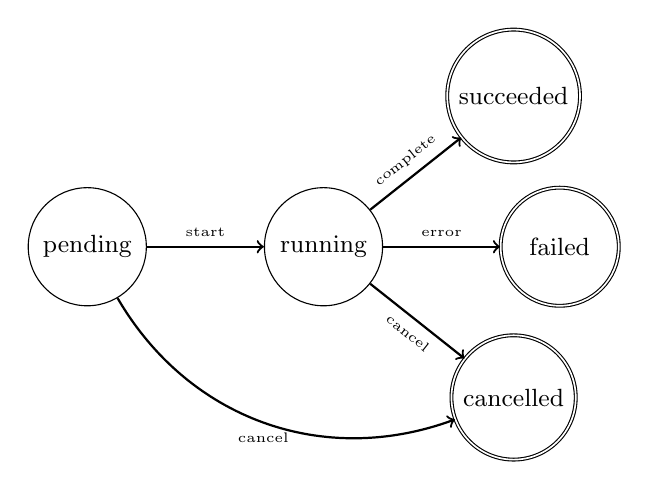
\begin{tikzpicture}[
    node distance=2cm,
    state/.style={circle, draw, minimum size=1.5cm, align=center, font=\small},
    final/.style={circle, draw, double, minimum size=1.5cm, align=center, font=\small},
    arrow/.style={->, thick}
]
    % States
    \node[state] (pending) {pending};
    \node[state, right of=pending, xshift=1cm] (running) {running};
    \node[final, above right of=running, xshift=1cm, yshift=0.5cm] (succeeded) {succeeded};
    \node[final, right of=running, xshift=1cm] (failed) {failed};
    \node[final, below right of=running, xshift=1cm, yshift=-0.5cm] (cancelled) {cancelled};
    
    % Transitions
    \draw[arrow] (pending) -- node[above, font=\tiny] {start} (running);
    \draw[arrow] (running) -- node[above, font=\tiny, sloped] {complete} (succeeded);
    \draw[arrow] (running) -- node[above, font=\tiny] {error} (failed);
    \draw[arrow] (running) -- node[below, font=\tiny, sloped] {cancel} (cancelled);
    \draw[arrow] (pending) edge[bend right=40] node[below, font=\tiny] {cancel} (cancelled);
\end{tikzpicture}
\caption{Agent run state machine}
\label{fig:run-state-machine}
\end{figure}

\begin{description}
    \item[pending] Initial state upon run creation. The run has been accepted but execution has not yet begun. Runs may be cancelled from this state.
    
    \item[running] Active execution state. The orchestrator is processing the request, invoking tools, and generating responses. Runs may transition to succeeded, failed, or cancelled.
    
    \item[succeeded] Terminal state indicating successful completion. The run produced valid output and all steps completed without errors.
    
    \item[failed] Terminal state indicating execution failure. An unrecoverable error occurred during processing.
    
    \item[cancelled] Terminal state indicating user or system cancellation. The run was terminated before completion, either by explicit request or timeout.
\end{description}

\subsection{End-to-End Request Flow}

The complete lifecycle of an agent run spans multiple system components, from HTTP request reception to final response delivery. Figure~\ref{fig:request-flow} illustrates this flow.

\begin{figure}[htbp]
\centering
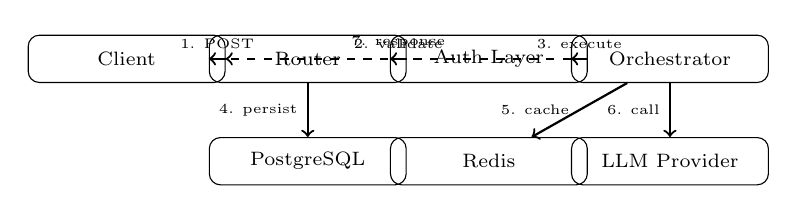
\begin{tikzpicture}[
    node distance=0.8cm,
    box/.style={rectangle, draw, rounded corners, minimum width=2.5cm, minimum height=0.6cm, align=center, font=\scriptsize},
    arrow/.style={->, thick}
]
    % Components
    \node[box] (client) {Client};
    \node[box, right of=client, xshift=1.5cm] (router) {Router};
    \node[box, right of=router, xshift=1.5cm] (auth) {Auth Layer};
    \node[box, right of=auth, xshift=1.5cm] (orch) {Orchestrator};
    
    \node[box, below of=router, yshift=-0.5cm] (db) {PostgreSQL};
    \node[box, below of=auth, yshift=-0.5cm] (redis) {Redis};
    \node[box, below of=orch, yshift=-0.5cm] (llm) {LLM Provider};
    
    % Flow arrows
    \draw[arrow] (client) -- node[above, font=\tiny] {1. POST} (router);
    \draw[arrow] (router) -- node[above, font=\tiny] {2. validate} (auth);
    \draw[arrow] (auth) -- node[above, font=\tiny] {3. execute} (orch);
    \draw[arrow] (router) -- node[left, font=\tiny] {4. persist} (db);
    \draw[arrow] (orch) -- node[left, font=\tiny] {5. cache} (redis);
    \draw[arrow] (orch) -- node[left, font=\tiny] {6. call} (llm);
    \draw[arrow, dashed] (orch) -- node[above, font=\tiny] {7. response} (client);
\end{tikzpicture}
\caption{Agent run request flow through system components}
\label{fig:request-flow}
\end{figure}

\subsubsection{Step 1: HTTP Request Reception}

The client submits a \texttt{POST} request to \texttt{/v1/agent-runs} with the following payload:

\begin{lstlisting}[language=Python, caption={Agent run request payload}, label=lst:run-request]
{
    "prompt": "How many :Blast nodes are in the graph?",
    "session_id": "uuid-optional",  # Optional session context
    "model": "phi3-mini-instruct",  # Optional model override
    "max_steps": 8,                  # Maximum execution steps
    "temperature": 0.2,              # LLM sampling temperature
    "metadata": {}                   # Arbitrary key-value data
}
\end{lstlisting}

\subsubsection{Step 2: Authentication and Authorization}

The router extracts and validates the JWT bearer token:

\begin{enumerate}
    \item Token signature verification against JWKS public keys
    \item Claims validation (issuer, audience, expiration)
    \item Principal construction with user ID, tenant ID, roles, and scopes
    \item Permission check for \texttt{agents:run} scope
\end{enumerate}

\subsubsection{Step 3: Run Creation and Persistence}

Upon successful authorization:

\begin{enumerate}
    \item A new run record is created with status \texttt{pending}
    \item The run is persisted to PostgreSQL via \texttt{AgentRunRepository}
    \item An event is logged to the audit trail
    \item The run ID is returned in the \texttt{202 Accepted} response
\end{enumerate}

\begin{lstlisting}[language=Python, caption={Run creation in router}, label=lst:run-creation]
# Create run record
run = AgentRun(
    run_id=uuid.uuid4(),
    session_id=session_id,
    user_id=user.sub,
    tenant_id=user.tenant_id,
    status="pending",
    input=request.prompt,
    model=request.model,
)
db.add(run)
db.commit()
\end{lstlisting}

\subsubsection{Step 4: Orchestrator Invocation}

The router invokes the orchestrator, either synchronously or via a background task:

\begin{lstlisting}[language=Python, caption={Orchestrator invocation}, label=lst:orch-invoke]
async def execute_agent_run_background(
    run_id: UUID,
    prompt: str,
    user_id: str,
    session_id: str,
    tenant_id: str,
    params: dict[str, Any],
):
    # Transition to running
    run.status = "running"
    db.commit()
    
    # Execute orchestration
    result = await orchestrator.run(
        goal=prompt,
        user_id=user_id,
        tenant_id=tenant_id,
        **params,
    )
    
    # Update with results
    run.status = "succeeded" if result.success else "failed"
    run.output = result.to_dict()
    db.commit()
\end{lstlisting}

\subsubsection{Step 5: Intent Classification and Routing}

The orchestrator classifies the prompt and routes to the appropriate handler:

\begin{enumerate}
    \item \texttt{classify\_intent()} analyzes the prompt
    \item Based on mode, the orchestrator invokes:
    \begin{itemize}
        \item \texttt{\_handle\_chat()} for CHAT mode
        \item \texttt{\_handle\_graph\_query()} for GRAPH mode
        \item \texttt{\_handle\_admin\_mode()} for ADMIN mode
        \item etc.
    \end{itemize}
\end{enumerate}

\subsubsection{Step 6: Step Execution Loop}

For complex requests, the orchestrator executes a planning and step execution loop:

\begin{enumerate}
    \item \textbf{TODO Planning}: Generate a list of steps to execute
    \item \textbf{Step Iteration}: For each TODO item:
    \begin{enumerate}
        \item Resolve the tool or action
        \item Prepare input parameters
        \item Execute with timeout
        \item Capture output and metrics
        \item Update step status
    \end{enumerate}
    \item \textbf{Result Aggregation}: Combine step outputs into final response
\end{enumerate}

\subsubsection{Step 7: Response Assembly and Delivery}

Upon completion:

\begin{enumerate}
    \item The \texttt{OrchestrationResult} is serialized to JSON
    \item The run record is updated with output and final status
    \item Metrics are emitted to Prometheus
    \item The response is returned to the client (for sync) or stored for polling (for async)
\end{enumerate}

\subsection{Polling and SSE Streaming}

For asynchronous runs, clients retrieve results via two mechanisms:

\paragraph{Polling} Clients may poll \texttt{GET /v1/agent-runs/\{id\}} to check run status and retrieve results:

\begin{lstlisting}[language=Python, caption={Run status response}, label=lst:run-status]
{
    "run_id": "uuid",
    "status": "running",  # pending | running | succeeded | failed | cancelled
    "progress": 0.5,       # Completion fraction (0.0-1.0)
    "output": null,        # Populated on completion
    "steps": [...],        # Executed steps so far
    "metrics": {...}       # Timing and usage metrics
}
\end{lstlisting}

\paragraph{SSE Streaming} For real-time progress, clients may subscribe to \texttt{GET /v1/agent-runs/\{id\}/events}:

\begin{lstlisting}[caption={SSE event stream}, label=lst:sse-stream]
event: status
data: {"status": "running", "step": 1, "total_steps": 3}

event: step_complete
data: {"step_id": "1", "action": "graph.generate_cypher", "latency_ms": 150}

event: status
data: {"status": "succeeded", "output": "There are 42 Blast nodes."}
\end{lstlisting}

\subsection{Agent Run Internal Structure}
\label{subsec:agent-run-internal-structure}

The agent run model comprises a hierarchy of entities: Sessions contain Runs, and Runs contain Steps. This structure enables conversational context, step-level auditability, and granular observability.

\subsubsection{Session Entity}

Sessions provide conversational context spanning multiple runs:

\begin{lstlisting}[language=Python, caption={Session schema fields}, label=lst:session-schema]
class SessionResponse(BaseModel):
    session_id: UUID           # Session identifier
    user_id: str               # Owner user ID
    tenant_id: str             # Tenant ID
    status: str                # active | completed | cancelled | failed
    manager: str | None        # Manager/planner LLM name
    preferred_workers: list[str] | None  # Preferred worker LLMs
    llm_preferences: dict[str, str] | None  # Tool -> LLM mapping
    agent_role: str | None     # Agent role (researcher, coder, etc.)
    tools: list[str] | None    # Allowed tools
    temperature: float         # Sampling temperature
    max_steps: int             # Maximum steps
    metadata: dict[str, Any]   # Arbitrary metadata
    created_at: datetime
    updated_at: datetime
    last_step_id: UUID | None  # Last step in session
\end{lstlisting}

Sessions enable:
\begin{itemize}
    \item Message history for context continuity across runs
    \item Per-session LLM and tool preferences
    \item Conversation state management
\end{itemize}

\subsubsection{Run Entity}

Runs represent single execution requests producing final output:

\begin{lstlisting}[language=Python, caption={Run response fields}, label=lst:run-schema]
class RunResponse(BaseModel):
    run_id: UUID              # Run identifier
    session_id: UUID | None   # Parent session
    user_id: str              # Owner user ID
    tenant_id: str            # Tenant ID
    status: str               # pending | running | succeeded | failed | cancelled
    model: str | None         # Model used
    manager: str | None       # Manager LLM
    input: str | None         # User prompt
    output: dict | None       # Final output
    steps: list[dict] | None  # Executed steps
    todos: list[dict] | None  # TODO items
    metrics: dict | None      # Execution metrics
    errors: list[str] | None  # Error messages
    warnings: list[str] | None  # Warning messages
    latency_ms: int | None    # Total execution time
    total_llm_calls: int | None  # LLM call count
    tool_calls: int | None    # Tool invocation count
    created_at: datetime
    finished_at: datetime | None
\end{lstlisting}

\subsubsection{Step Entity}

Steps represent individual units of work within a run:

\begin{lstlisting}[language=Python, caption={Step schema fields}, label=lst:step-schema]
class StepResponse(BaseModel):
    step_id: UUID             # Step identifier
    session_id: UUID          # Parent session
    seq: int                  # Sequence number
    type: str                 # message | user | assistant | tool | system | error
    message: str | None       # Human-readable message
    tool: str | None          # Tool name (if tool step)
    input: dict | None        # Input payload
    output: dict | None       # Output payload
    status: str               # queued | running | completed | failed | cancelled
    error: dict | None        # Error details
    created_at: datetime
    completed_at: datetime | None
\end{lstlisting}

Step types include:
\begin{itemize}
    \item \texttt{message}: User message input
    \item \texttt{assistant}: LLM-generated response
    \item \texttt{tool}: Tool invocation with input/output
    \item \texttt{system}: System-generated message
    \item \texttt{error}: Error occurrence
\end{itemize}

\subsubsection{TODO Item Entity}

TODO items represent the planning phase output:

\begin{lstlisting}[language=Python, caption={TodoItem schema}, label=lst:todo-schema]
class TodoItem(BaseModel):
    task: str                 # Task description
    status: str               # pending | in_progress | done | skipped
    order: int | None         # Execution order
    meta: dict | None         # Additional metadata
\end{lstlisting}

The orchestrator generates TODO items during planning, then iterates through them during execution, updating status as each completes.

\subsubsection{Orchestration Step Input/Output}

The orchestrator uses typed dataclasses for step tracking:

\begin{lstlisting}[language=Python, caption={OrchestrationStepInput schema}, label=lst:orch-step-input]
class OrchestrationStepInput(BaseModel):
    type: Literal["step"] = "step"
    step_id: str              # Step identifier
    action: str               # Action/tool to execute
    input: dict | None        # Input parameters
    started_at: datetime | None
    finished_at: datetime | None
    latency_ms: int | None    # Calculated from timestamps
\end{lstlisting}

\begin{lstlisting}[language=Python, caption={OrchestrationStepOutput schema}, label=lst:orch-step-output]
class OrchestrationStepOutput(BaseModel):
    type: Literal["output"] = "output"
    step_id: str              # Matching input step
    output: dict | None       # Output data
    error: str | None         # Error message if failed
    started_at: datetime | None
    finished_at: datetime | None
    latency_ms: int | None
\end{lstlisting}

The schemas include automatic latency calculation from timestamps, ensuring timing consistency across the system.

\subsection{Persistence and Caching Strategy}

The agent run lifecycle leverages a dual-storage approach:

\paragraph{PostgreSQL (Control Plane)} Authoritative storage for:
\begin{itemize}
    \item Run records with complete history
    \item Step records with input/output payloads
    \item Session state and configuration
    \item Audit trail entries
\end{itemize}

\paragraph{Redis (Data Plane)} Ephemeral storage for:
\begin{itemize}
    \item Session state caching for fast access
    \item Step sequence counters (\texttt{allocate\_next\_seq})
    \item Session locks for concurrent access control
    \item Cancellation flags
    \item ETag invalidation markers
\end{itemize}

\begin{lstlisting}[language=Python, caption={Redis session state functions}, label=lst:redis-session]
# Session state management
def get_session_state(session_id: str) -> dict | None:
    """Get cached session state from Redis."""
    
def set_session_state(session_id: str, state: dict, ttl: int = 3600):
    """Cache session state in Redis with TTL."""
    
def set_session_cancelled(session_id: str):
    """Mark session as cancelled in Redis."""
    
def session_lock(session_id: str, timeout: int = 30):
    """Acquire distributed lock for session modification."""
\end{lstlisting}

\subsection{Metrics and Observability Integration}

Each stage of the run lifecycle emits metrics for monitoring:

\begin{table}[htbp]
\centering
\caption{Agent run metrics}
\label{tab:run-metrics}
\begin{tabular}{lll}
\hline
\textbf{Metric} & \textbf{Type} & \textbf{Description} \\
\hline
\texttt{agent\_runs\_total} & Counter & Total runs by status, tenant \\
\texttt{agent\_run\_duration\_seconds} & Histogram & Run duration by intent type \\
\texttt{agent\_run\_steps\_total} & Counter & Steps executed \\
\texttt{agent\_run\_tokens\_total} & Counter & LLM tokens consumed \\
\texttt{agent\_run\_tool\_calls\_total} & Counter & Tool invocations \\
\texttt{agent\_run\_errors\_total} & Counter & Errors by type \\
\hline
\end{tabular}
\end{table}

Structured logging with \texttt{structlog} provides correlation IDs linking log entries across the run lifecycle:

\begin{lstlisting}[language=Python, caption={Structured logging example}, label=lst:structured-log]
log.info(
    "agent_run.started",
    run_id=str(run_id),
    user_id=user_id,
    tenant_id=tenant_id,
    intent_mode=intent.mode,
    intent_confidence=intent.confidence,
)
\end{lstlisting}

\subsection{Error Handling and Recovery}

The run lifecycle implements comprehensive error handling:

\subsubsection{Error Classification}

Errors are classified by type for appropriate handling:

\begin{lstlisting}[language=Python, caption={LLM error classification}, label=lst:error-classification]
def classify_llm_error(error_message: str) -> str:
    """Classify LLM error type from error message."""
    msg_lower = error_message.lower()
    
    if "timeout" in msg_lower:
        return "timeout"
    elif "context length" in msg_lower:
        return "context_length"
    elif "rate limit" in msg_lower:
        return "rate_limit"
    elif "connection" in msg_lower:
        return "connection"
    elif "validation" in msg_lower:
        return "validation"
    else:
        return "unknown"
\end{lstlisting}

\subsubsection{Graceful Degradation}

When errors occur, the orchestrator attempts graceful degradation:

\begin{enumerate}
    \item \textbf{Retry with backoff}: Transient errors trigger retry with exponential backoff
    \item \textbf{Fallback providers}: LLM failures may trigger fallback to alternative providers
    \item \textbf{Partial results}: If some steps succeed, partial results are preserved
    \item \textbf{Deterministic fallback}: For certain query patterns, deterministic responses replace LLM calls
\end{enumerate}

\subsubsection{Cancellation Handling}

Runs support cooperative cancellation:

\begin{enumerate}
    \item Client sends \texttt{DELETE /v1/agent-runs/\{id\}}
    \item Cancellation flag is set in Redis
    \item Orchestrator checks flag between steps
    \item If set, orchestrator halts execution and transitions to \texttt{cancelled}
    \item Partial results are preserved for debugging
\end{enumerate}

This design ensures that long-running operations can be interrupted without leaving the system in an inconsistent state.

